% fig2_color_body.tex: modeled color body and its achromatic quotient.
% Standalone vector drawing. Build: pdflatex fig2_color_body.tex
\documentclass[tikz,border=6pt]{standalone}
\usepackage[T1]{fontenc}
\usepackage{lmodern}
\usepackage{amsmath,amssymb}
\usepackage{xcolor}
\usetikzlibrary{arrows.meta,positioning,calc}
\begin{document}
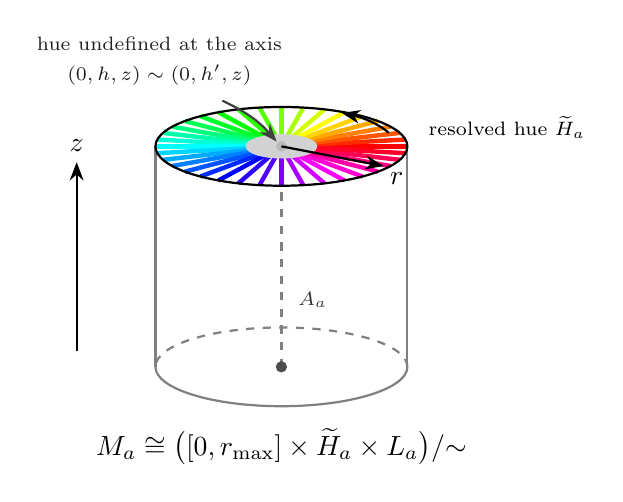
\begin{tikzpicture}[>=Stealth, line width=0.8pt]

  \draw[dashed, gray] (1.6,-1.4) arc[start angle=0, end angle=180,
    x radius=1.6, y radius=0.5];
  \draw[gray] (1.6,-1.4) arc[start angle=0, end angle=-180,
    x radius=1.6, y radius=0.5];
  \draw[gray] (-1.6,-1.4) -- (-1.6,1.4);
  \draw[gray] ( 1.6,-1.4) -- ( 1.6,1.4);
  \draw[gray, dashed] (0,-1.4) -- (0,1.4);
  \filldraw[gray!60!black] (0,-1.4) circle (1.6pt);

  \foreach \k in {0,...,35}{
    \pgfmathsetmacro{\hue}{\k/36}
    \pgfmathsetmacro{\ang}{\k*10}
    \definecolor{spokecol}{hsb}{\hue,1,1}
    \draw[spokecol, line width=1.6pt]
      (0,1.4) -- ({1.6*cos(\ang)},{1.4+0.5*sin(\ang)});
  }
  \filldraw[gray!35] (0,1.4) ellipse[x radius=0.44, y radius=0.14];
  \filldraw[gray!55!white] (0,1.4) circle (1.5pt);
  \draw (0,1.4) ellipse[x radius=1.6, y radius=0.5];

  \draw[->] (-2.6,-1.2) -- (-2.6,1.2);
  \node[above] at (-2.6,1.2) {$z$};
  \draw[->, black] (0,1.4) -- ({1.5*cos(-30)},{1.4+0.5*sin(-30)});
  \node[below right=-2pt] at ({1.5*cos(-30)},{1.4+0.5*sin(-30)}) {$r$};
  \draw[->, black] ({1.45*cos(20)},{1.4+0.5*sin(20)})
    arc[start angle=20, end angle=58, x radius=1.45, y radius=0.5];
  \node[right] at (1.74,1.64) {\scriptsize resolved hue $\widetilde H_a$};
  \node[right=1pt, gray!40!black] at (0.05,-0.55) {\scriptsize $A_a$};

  \draw[->, gray!50!black] (-0.75,1.98) to[bend left=12] (-0.06,1.46);
  \node[anchor=south, align=center, gray!25!black] at (-1.55,2.04)
    {\scriptsize hue undefined at the axis\\[-1pt]
     \scriptsize $(0,h,z)\sim(0,h',z)$};

  \node[anchor=north] at (0,-2.05)
    {$M_a\cong\bigl([0,r_{\max}]\times\widetilde H_a\times L_a\bigr)/{\sim}$};

\end{tikzpicture}
\end{document}
